% fig_montecarlo.tex — fragment (\input-able, no standalone wrapper)
\pgfplotsset{compat=1.18}
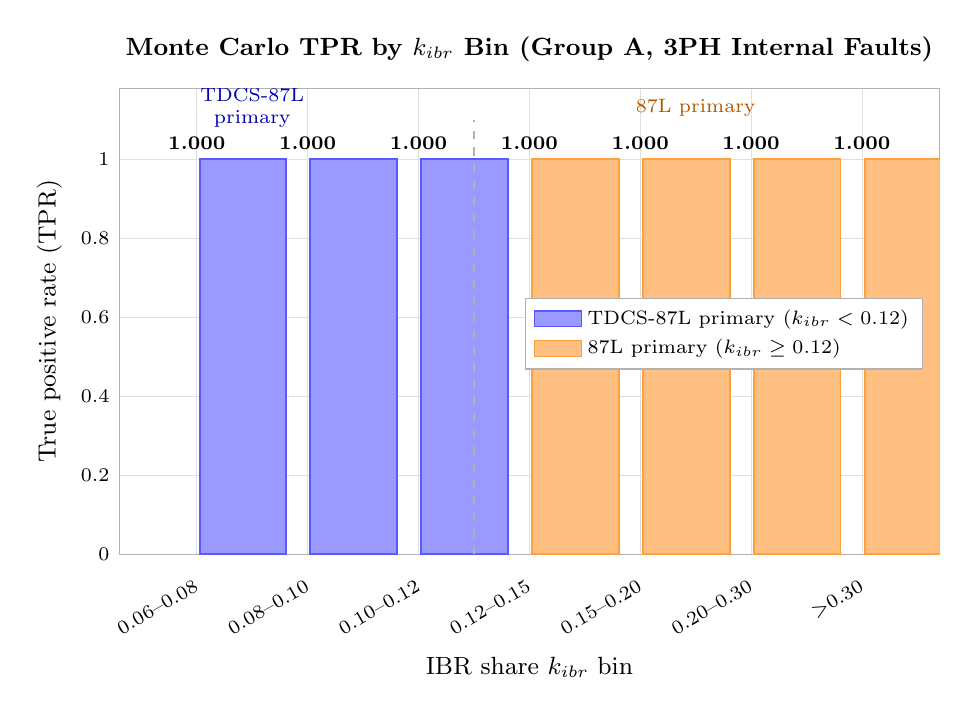
\begin{tikzpicture}
\begin{axis}[
  width=12cm, height=7.5cm,
  title={Monte Carlo TPR by $k_{ibr}$ Bin (Group A, 3PH Internal Faults)},
  title style={font=\small\bfseries},
  ybar,
  bar width=1.1cm,
  xlabel={IBR share $k_{ibr}$ bin},
  ylabel={True positive rate (TPR)},
  xlabel style={font=\small},
  ylabel style={font=\small},
  xtick={1,2,3,4,5,6,7},
  xticklabels={%
    {0.06--0.08},
    {0.08--0.10},
    {0.10--0.12},
    {0.12--0.15},
    {0.15--0.20},
    {0.20--0.30},
    {$>$0.30}},
  xticklabel style={font=\scriptsize, rotate=30, anchor=north east},
  xmin=0.3, xmax=7.7,
  ymin=0, ymax=1.18,
  ytick={0, 0.2, 0.4, 0.6, 0.8, 1.0},
  yticklabel style={font=\scriptsize},
  grid=both,
  grid style={gray!25, line width=0.3pt},
  tick style={draw=none},
  axis line style={gray!60},
  legend style={at={(0.98,0.55)}, anchor=north east,
                font=\scriptsize, draw=gray!60,
                cells={anchor=west}},
]

% ---- TDCS-primary bins (k_ibr < 0.12): bins 1, 2, 3 ------------------------
\addplot[fill=blue!40, draw=blue!65, line width=0.7pt,
         forget plot] coordinates {
  (1, 1.000)
  (2, 1.000)
  (3, 1.000)
};

% ---- 87L-primary bins (k_ibr >= 0.12): bins 4, 5, 6, 7 --------------------
\addplot[fill=orange!50, draw=orange!75, line width=0.7pt,
         forget plot] coordinates {
  (4, 1.000)
  (5, 1.000)
  (6, 1.000)
  (7, 1.000)
};

% ---- Legend proxies ---------------------------------------------------------
\addlegendimage{area legend, fill=blue!40,  draw=blue!65}
\addlegendentry{TDCS-87L primary ($k_{ibr}<0.12$)}
\addlegendimage{area legend, fill=orange!50, draw=orange!75}
\addlegendentry{87L primary ($k_{ibr}\geq 0.12$)}

% ---- TPR=1.000 labels above each bar ----------------------------------------
\node[font=\scriptsize\bfseries, above] at (axis cs:1, 1.000) {1.000};
\node[font=\scriptsize\bfseries, above] at (axis cs:2, 1.000) {1.000};
\node[font=\scriptsize\bfseries, above] at (axis cs:3, 1.000) {1.000};
\node[font=\scriptsize\bfseries, above] at (axis cs:4, 1.000) {1.000};
\node[font=\scriptsize\bfseries, above] at (axis cs:5, 1.000) {1.000};
\node[font=\scriptsize\bfseries, above] at (axis cs:6, 1.000) {1.000};
\node[font=\scriptsize\bfseries, above] at (axis cs:7, 1.000) {1.000};

% ---- Region divider at boundary between bin 3 and bin 4 --------------------
\draw[gray!60, dashed, line width=0.9pt]
  (axis cs:3.5, 0) -- (axis cs:3.5, 1.10);

% ---- Region annotation labels -----------------------------------------------
\node[font=\scriptsize, blue!70!black, align=center]
  at (axis cs:1.5, 1.13) {TDCS-87L\\primary};
\node[font=\scriptsize, orange!70!black, align=center]
  at (axis cs:5.5, 1.13) {87L primary};

\end{axis}
\end{tikzpicture}
